\section{Histograms on the Second Run~\label{sec:sodb9_r2_hist}} 
This section exhibits histograms on the second run of 
INC with its task length increasing from 1 second to 4096 seconds, via EMPv5. 
The detailed description of the base data is from Table~\ref{tab:exp_notes}.

\subsection{ET}

\begin{figure}[hp!]
	\centering
	\subfigure[ET frequency on INC1]{
		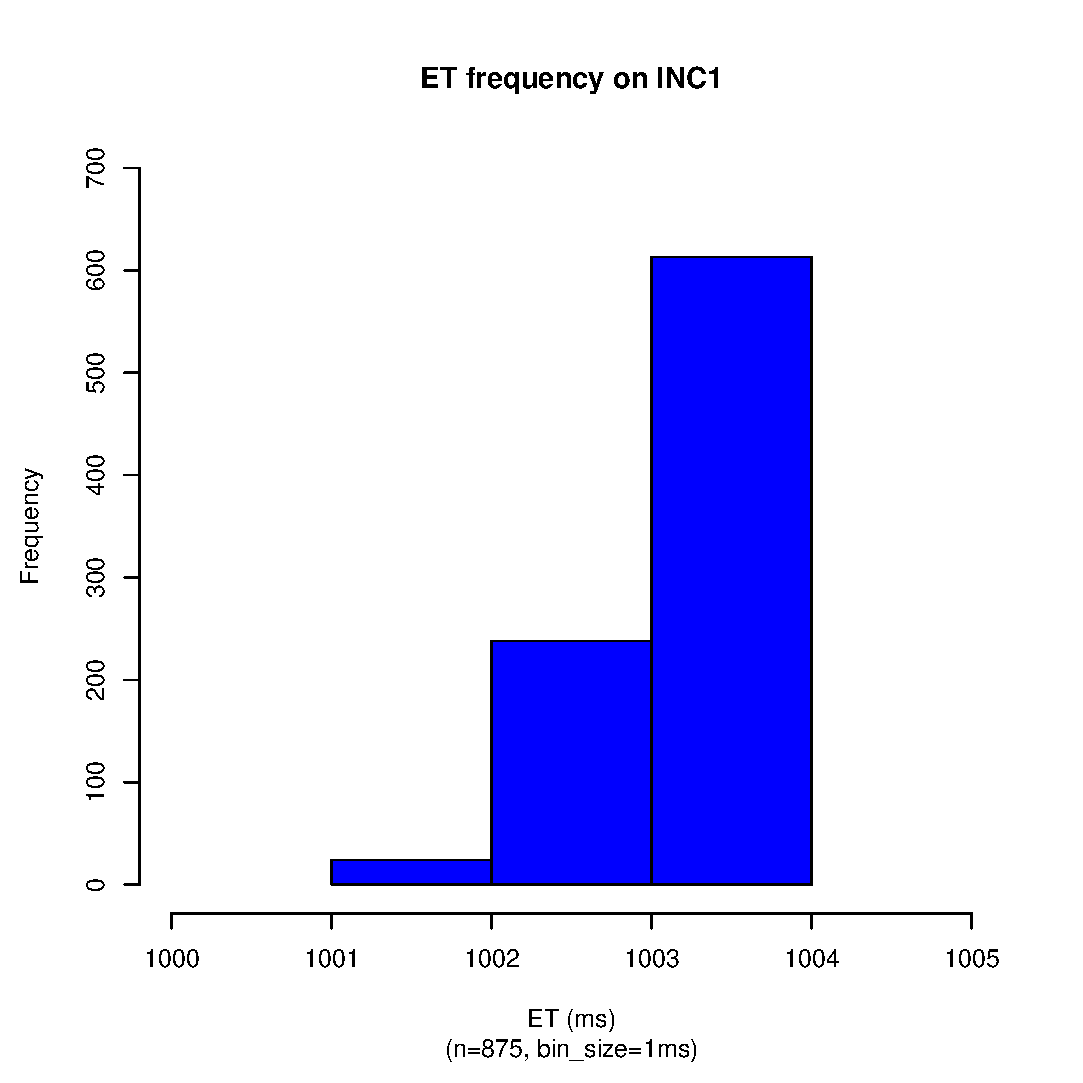
\includegraphics[scale=0.43]{repet_data1/1_sec_et_hist_v5.eps}
		\label{fig:inc1_r2_et_hist_v5}
	}
	\subfigure[ET frequency on INC2]{
		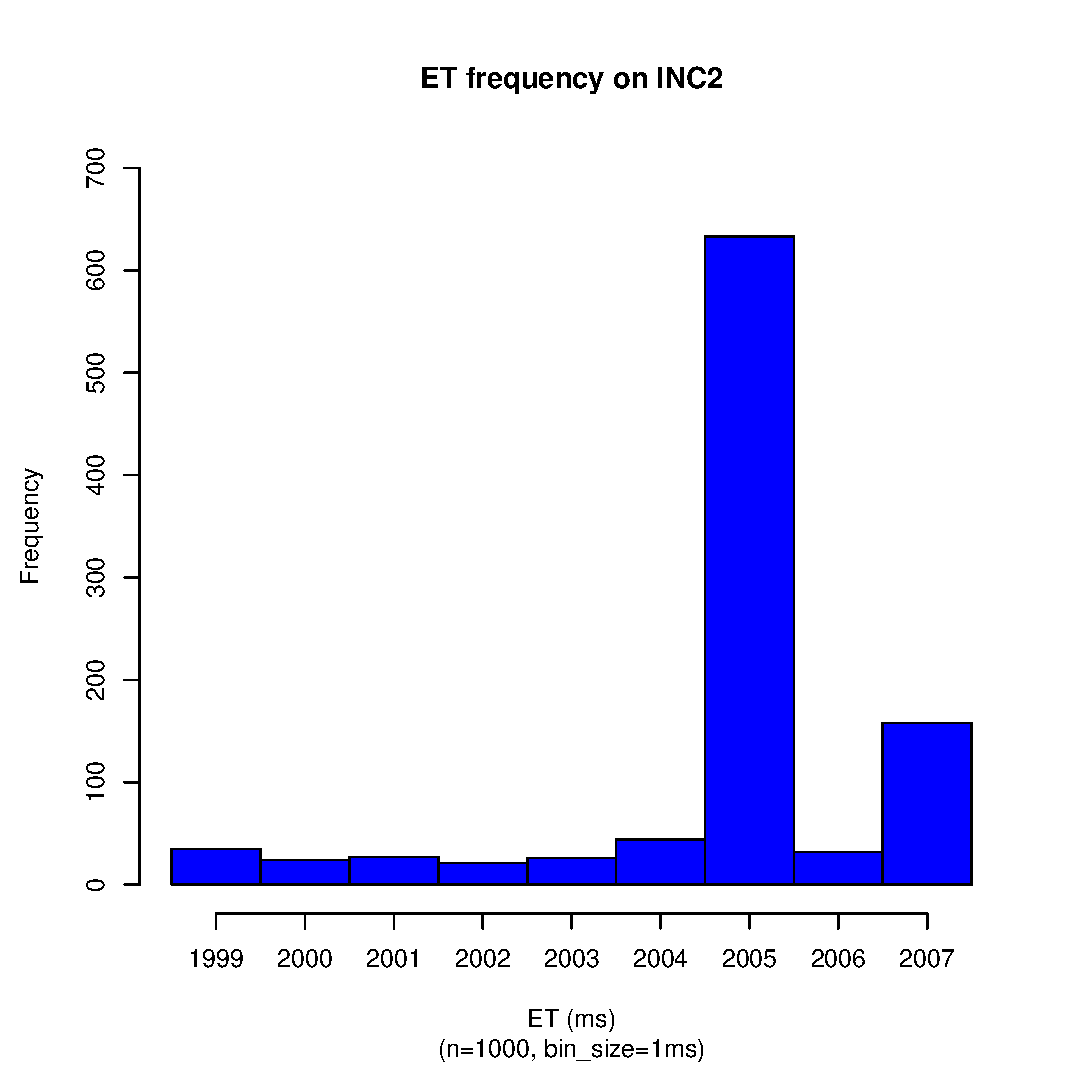
\includegraphics[scale=0.43]{repet_data2/2_sec_et_hist_v5.eps}
		\label{fig:inc2_r2_et_hist_v5}
	}
	\subfigure[ET frequency on INC4]{
		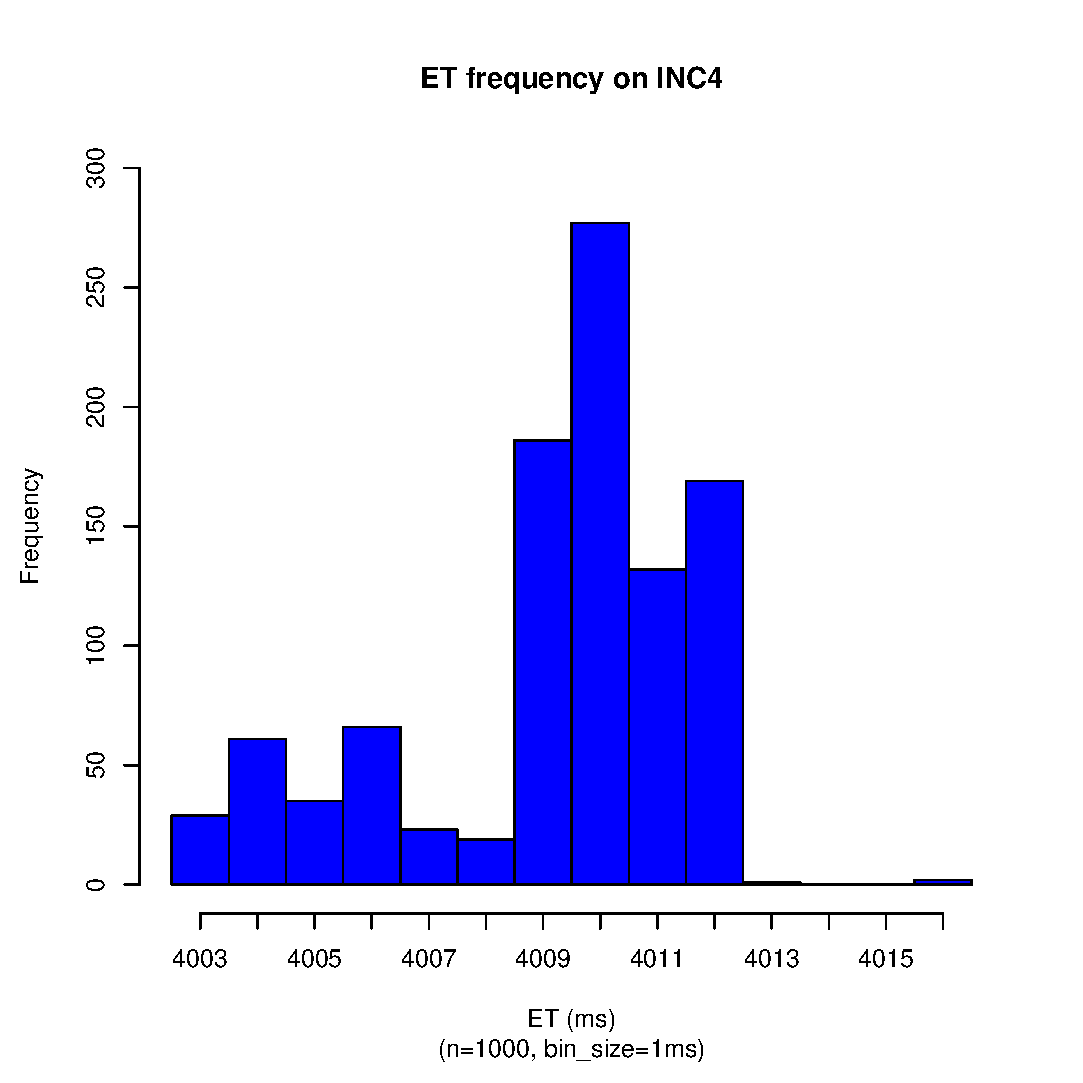
\includegraphics[scale=0.43]{repet_data2/4_sec_et_hist_v5.eps}
		\label{fig:inc4_r2_et_hist_v5}
	}
	\subfigure[ET frequency on INC8]{
		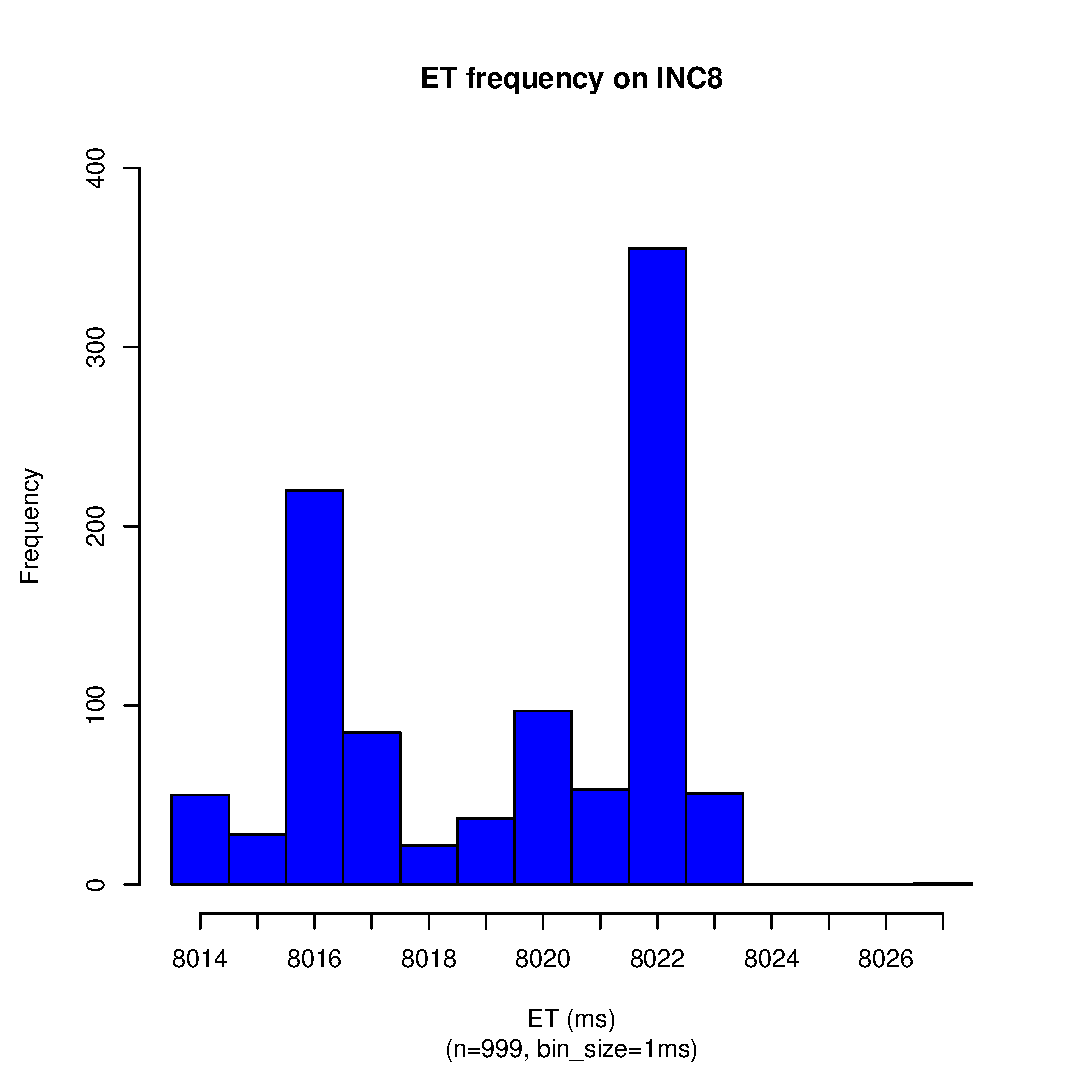
\includegraphics[scale=0.43]{repet_data2/8_sec_et_hist_v5.eps}
		\label{fig:inc8_r2_et_hist_v5}
	}
	\caption{ET Histograms of INC1 ... INC8~\label{fig:s9_r2_et_hist1}}
\end{figure}

\begin{figure}[hp!]
	\centering
	\subfigure[ET frequency on INC16]{
		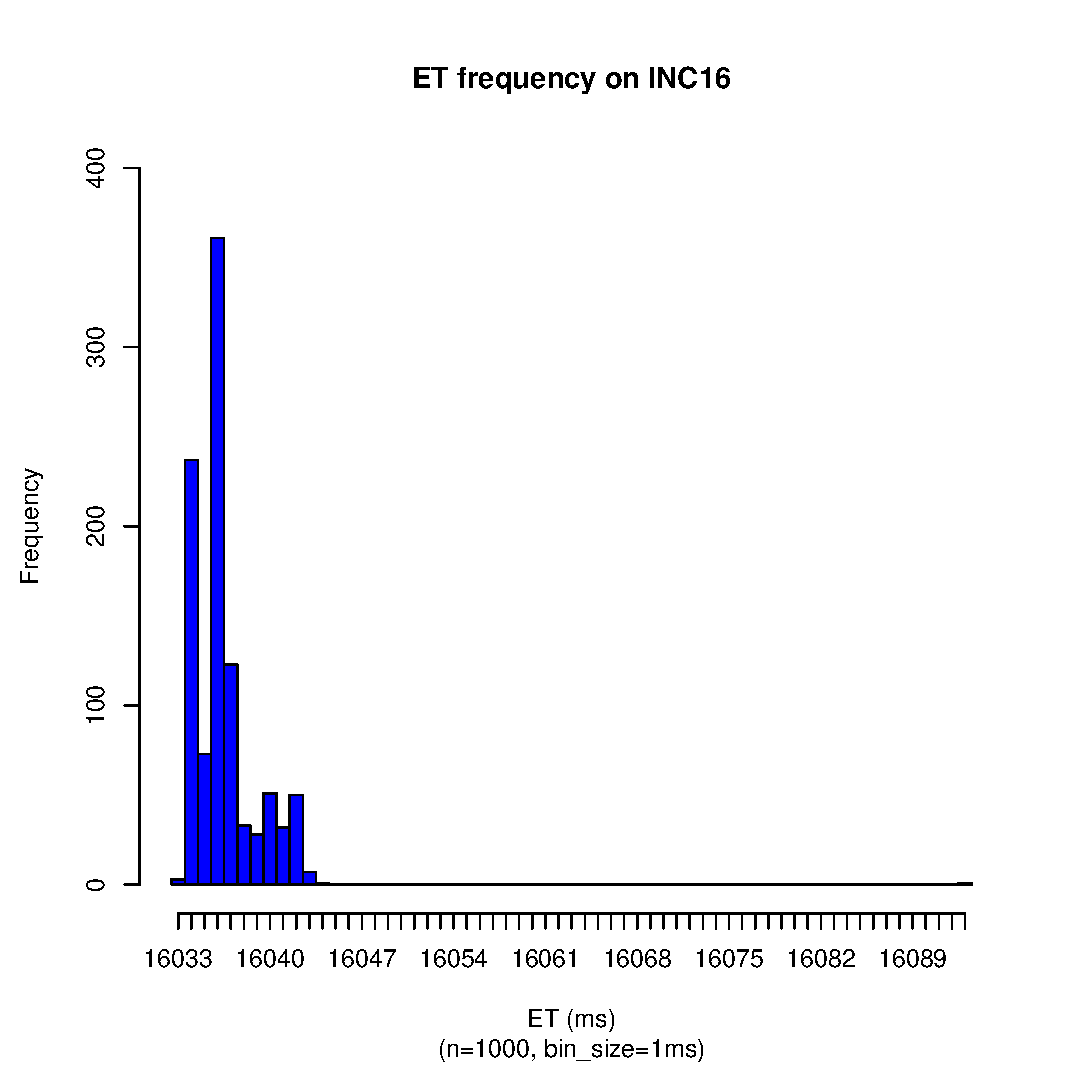
\includegraphics[scale=0.43]{repet_data2/16_sec_et_hist_v5.eps}
		\label{fig:inc16_r2_et_hist_v5}
	}
	\subfigure[ET frequency on INC32]{
		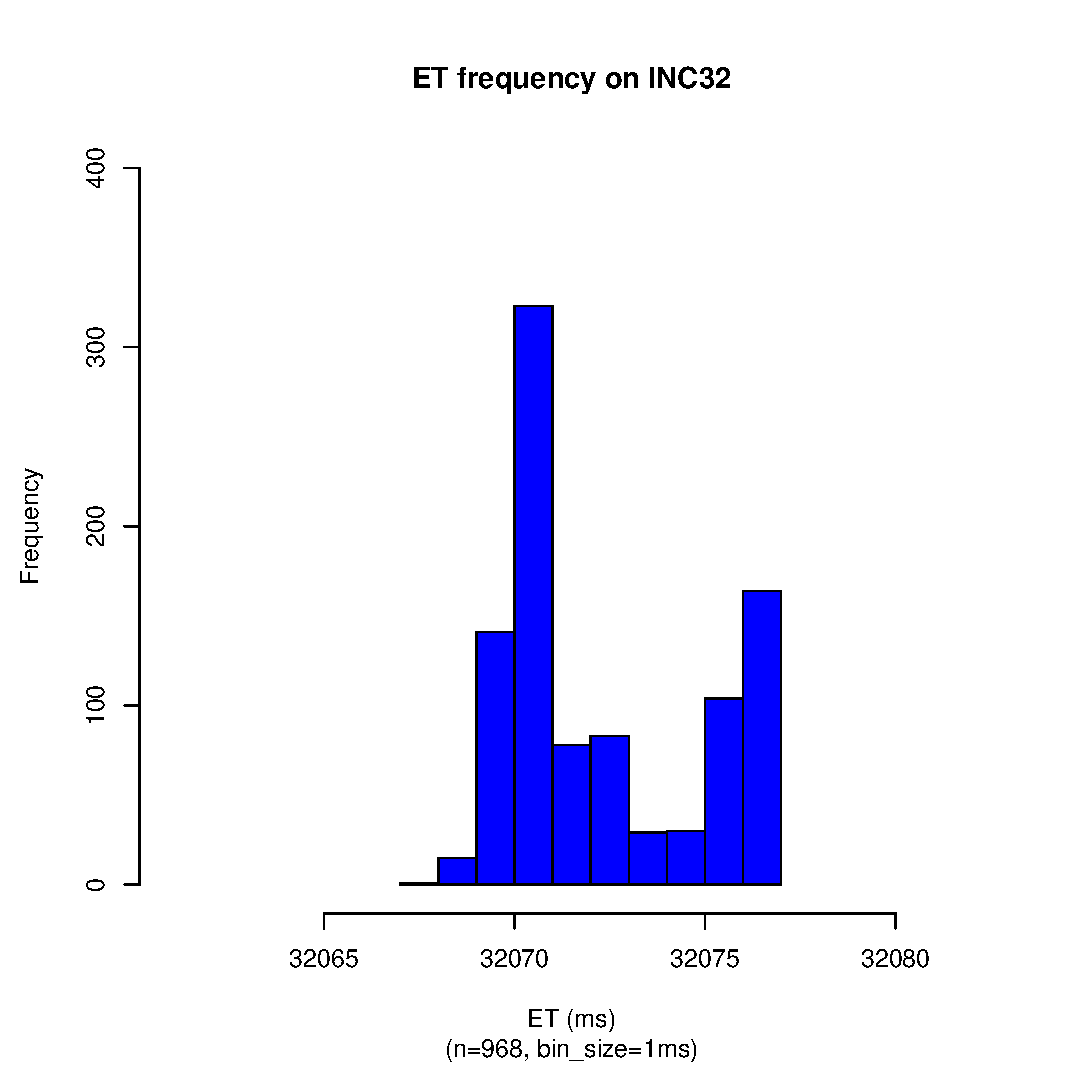
\includegraphics[scale=0.43]{repet_data2/32_sec_et_hist_v5.eps}
		\label{fig:inc32_r2_et_hist_v5}
	}
	\subfigure[ET frequency on INC64]{
		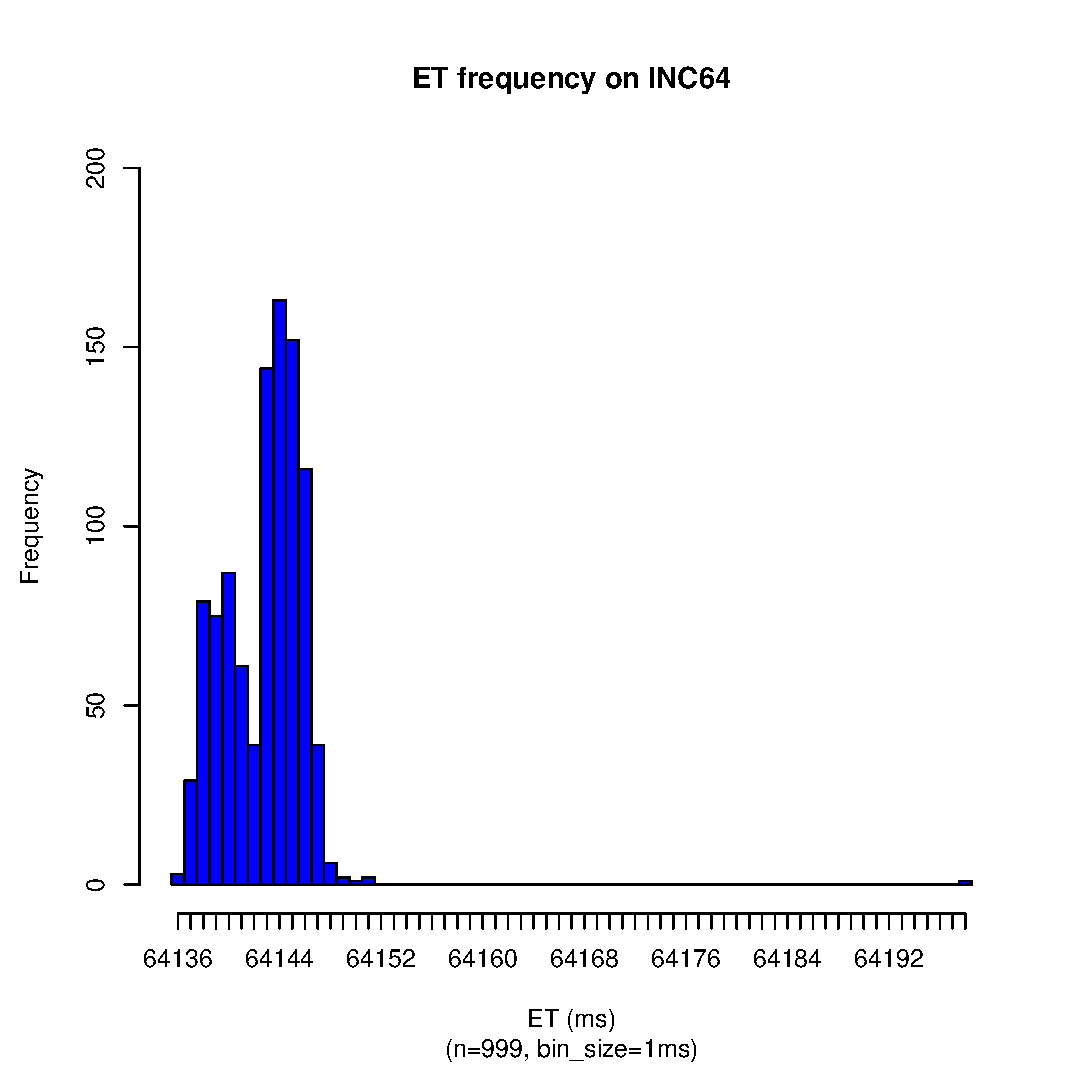
\includegraphics[scale=0.43]{repet_data2/64_sec_et_hist_v5.eps}
		\label{fig:inc64_r2_et_hist_v5}
	}
	\caption{ET Histograms of INC16 ... INC64~\label{fig:s9_r2_et_hist2}}
\end{figure}

\begin{figure}[hp!]
	\centering
	\subfigure[ET frequency on INC128]{
		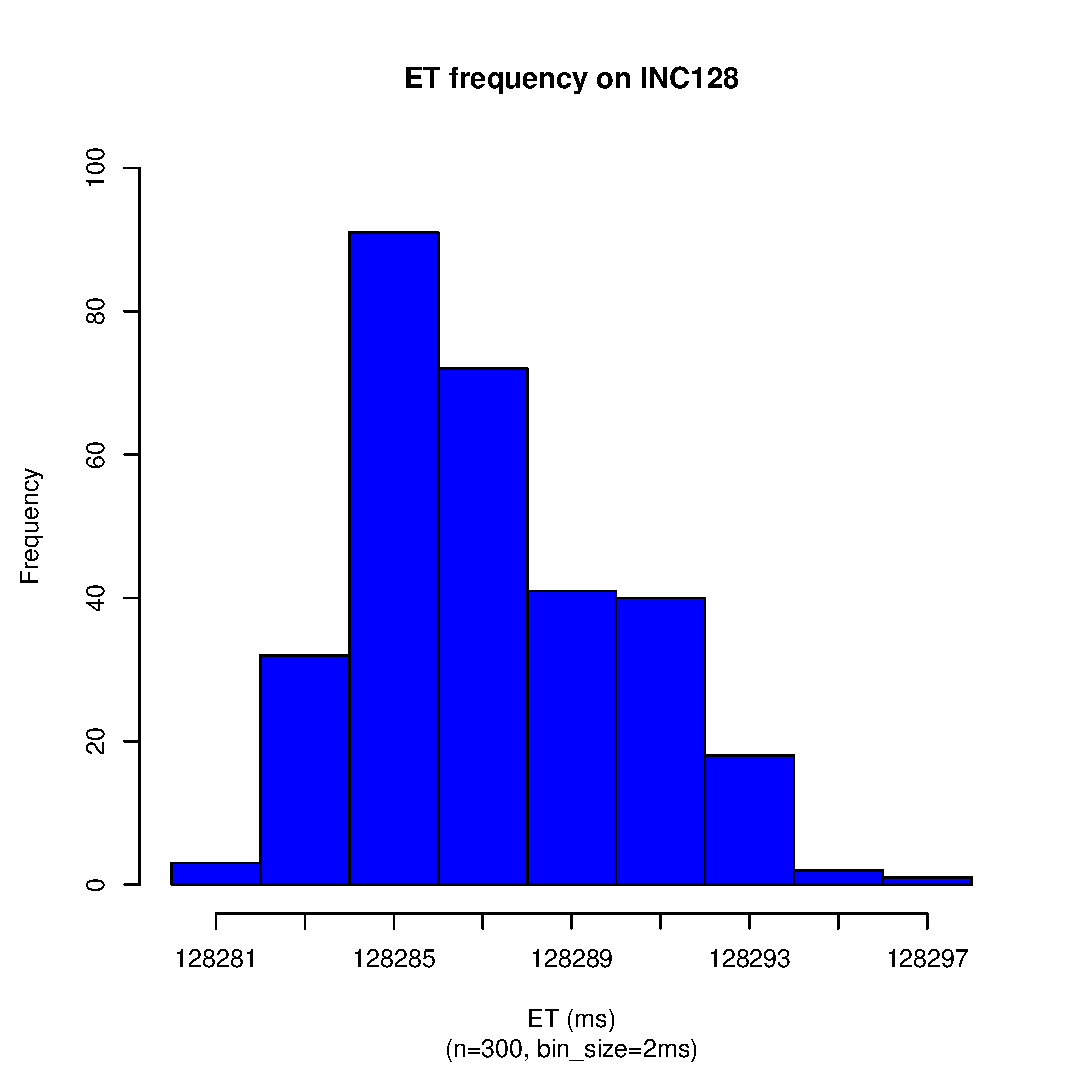
\includegraphics[scale=0.43]{repet_data2/128_sec_et_hist_v5.eps}
		\label{fig:inc128_r2_et_hist_v5}
	}
	\subfigure[ET frequency on INC256]{
		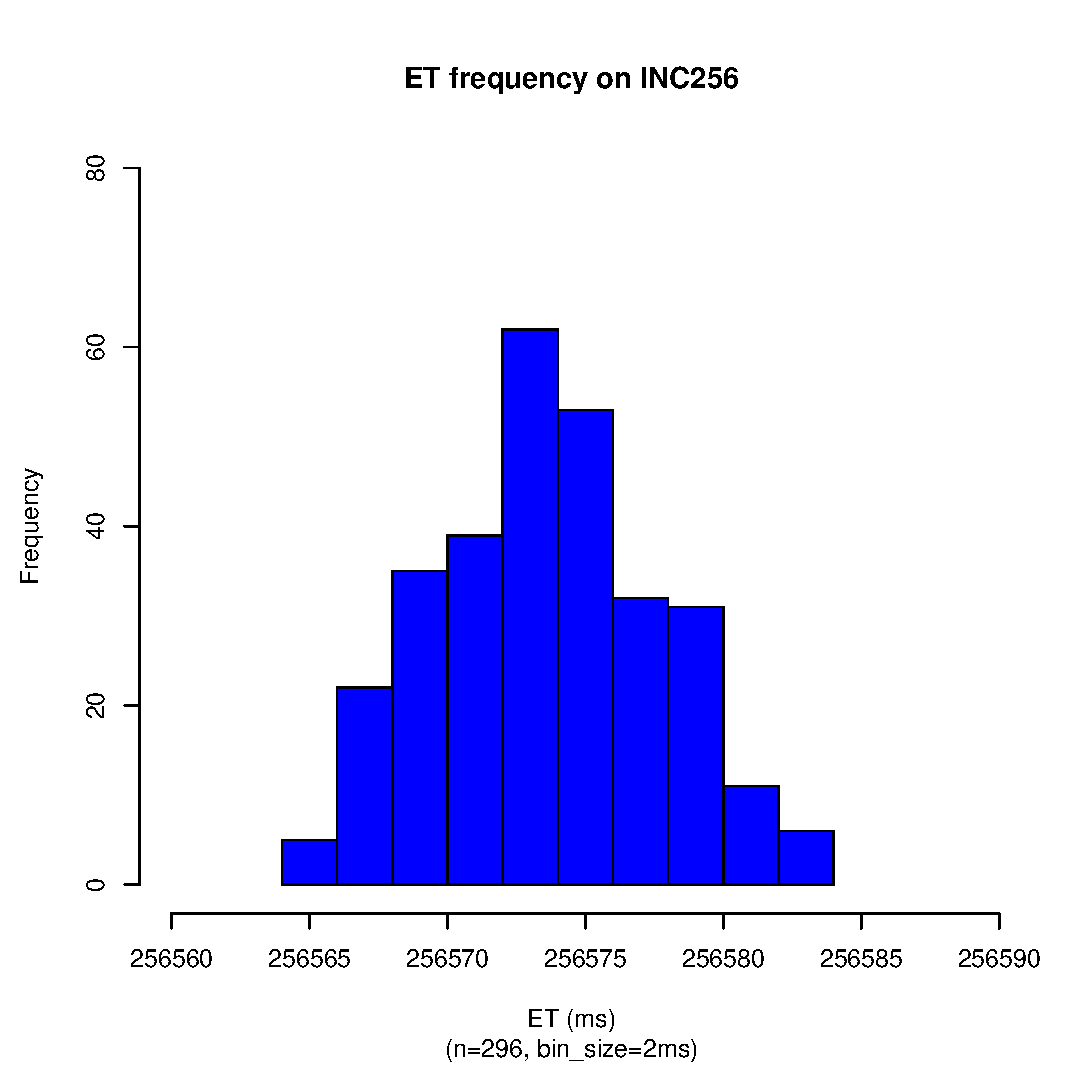
\includegraphics[scale=0.43]{repet_data2/256_sec_et_hist_v5.eps}
		\label{fig:inc256_r2_et_hist_v5}
	}
	\subfigure[ET frequency on INC512]{
		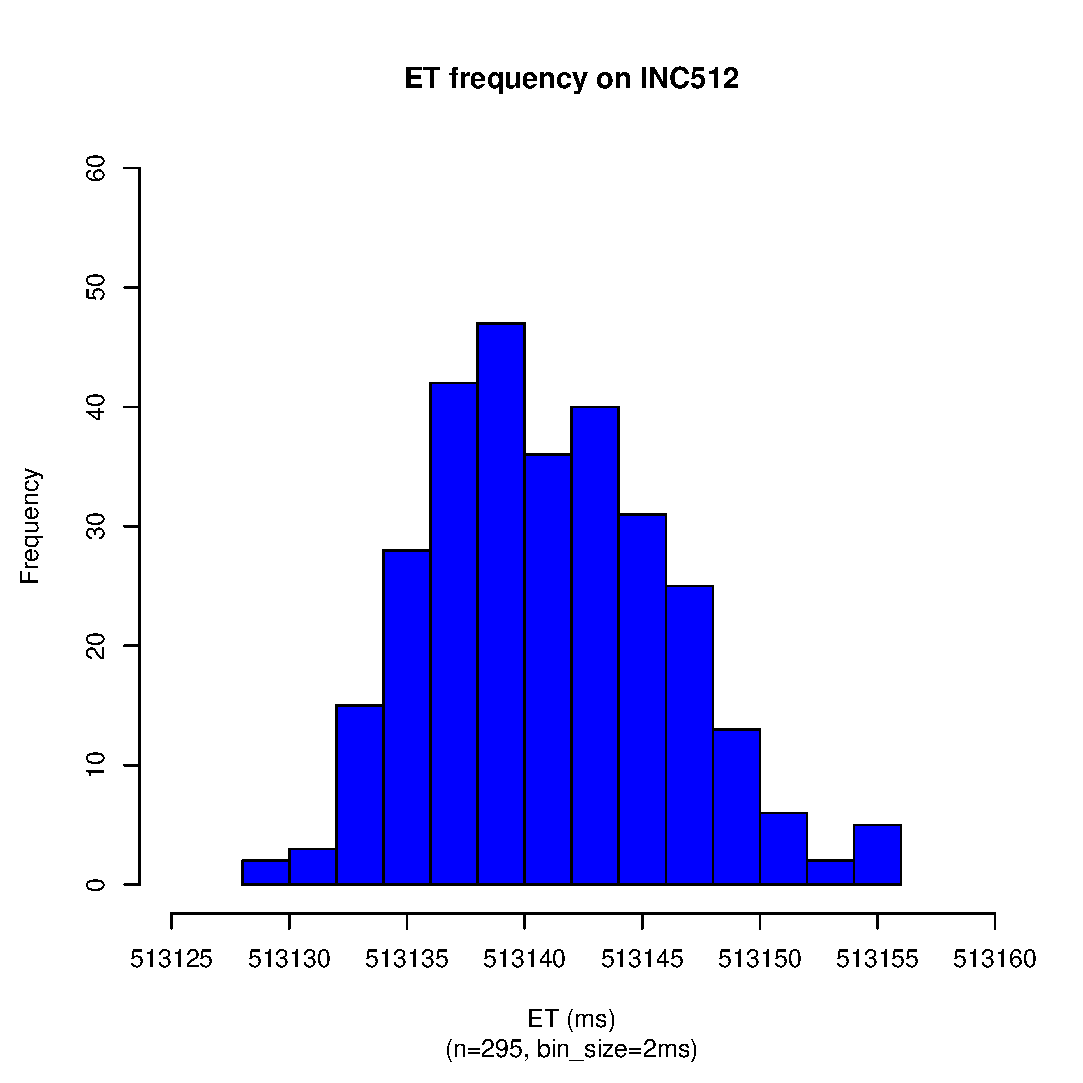
\includegraphics[scale=0.43]{repet_data2/512_sec_et_hist_v5.eps}
		\label{fig:inc512_r2_et_hist_v5}
	}
	\subfigure[ET frequency on INC1024]{
		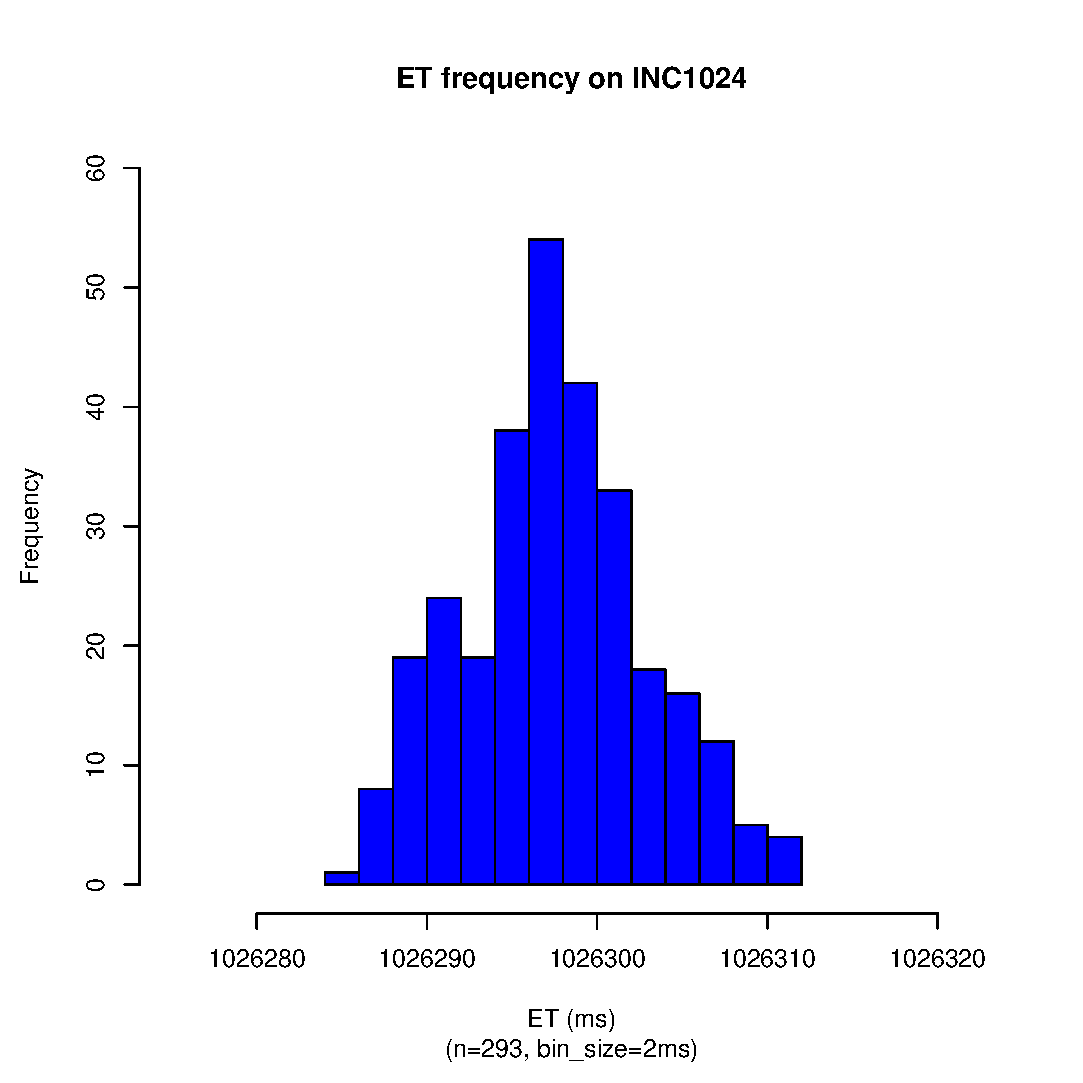
\includegraphics[scale=0.43]{repet_data2/1024_sec_et_hist_v5.eps}
		\label{fig:inc1024_r2_et_hist_v5}
	}
	\caption{ET Histograms of INC128 ... INC1024~\label{fig:s9_r2_et_hist3}}
\end{figure}

\begin{figure}[hp!]
	\centering
	\subfigure[ET frequency on INC2048]{
		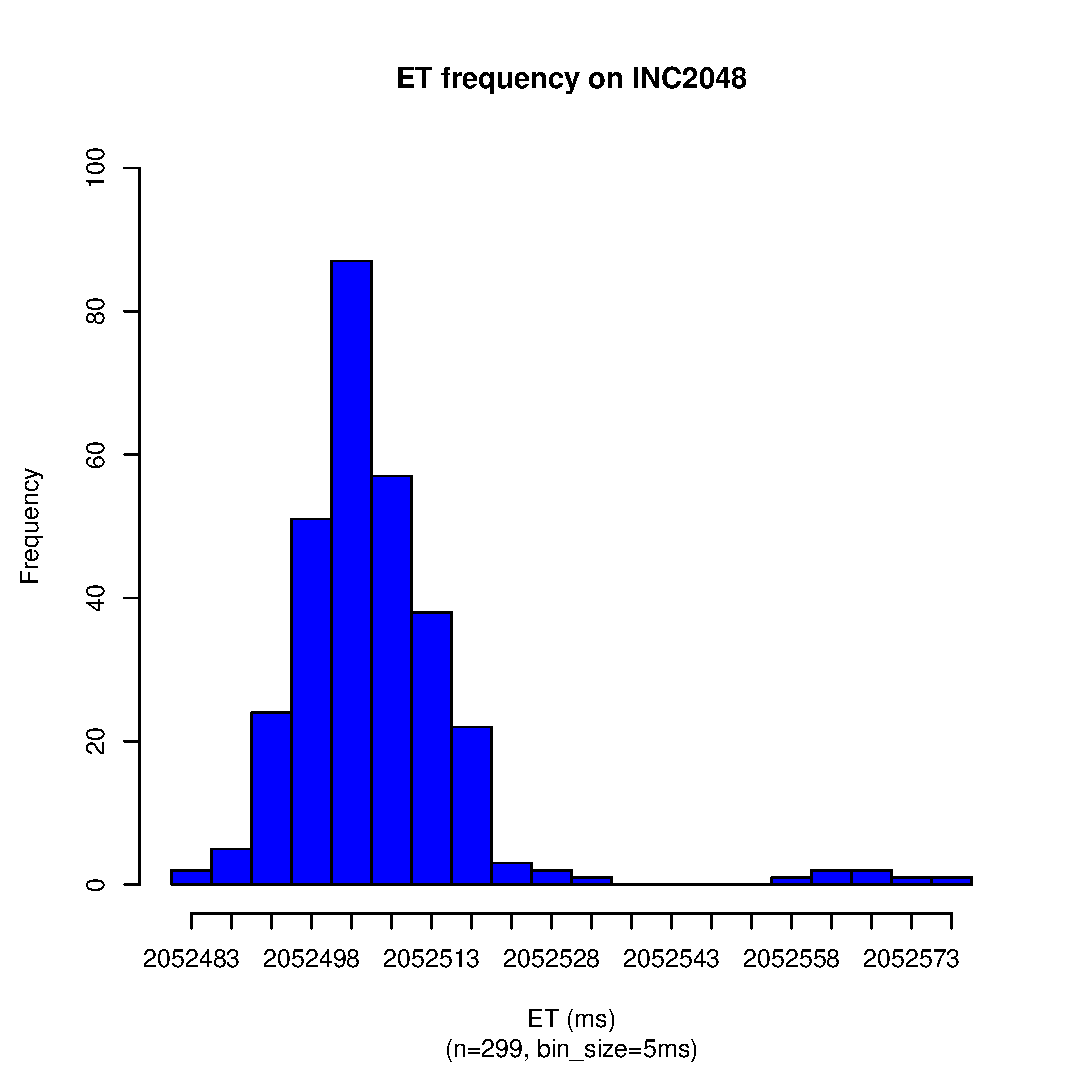
\includegraphics[scale=0.43]{repet_data2/2048_sec_et_hist_v5.eps}
		\label{fig:inc2048_r2_et_hist_v5}
	}
	\subfigure[ET frequency on INC4096]{
		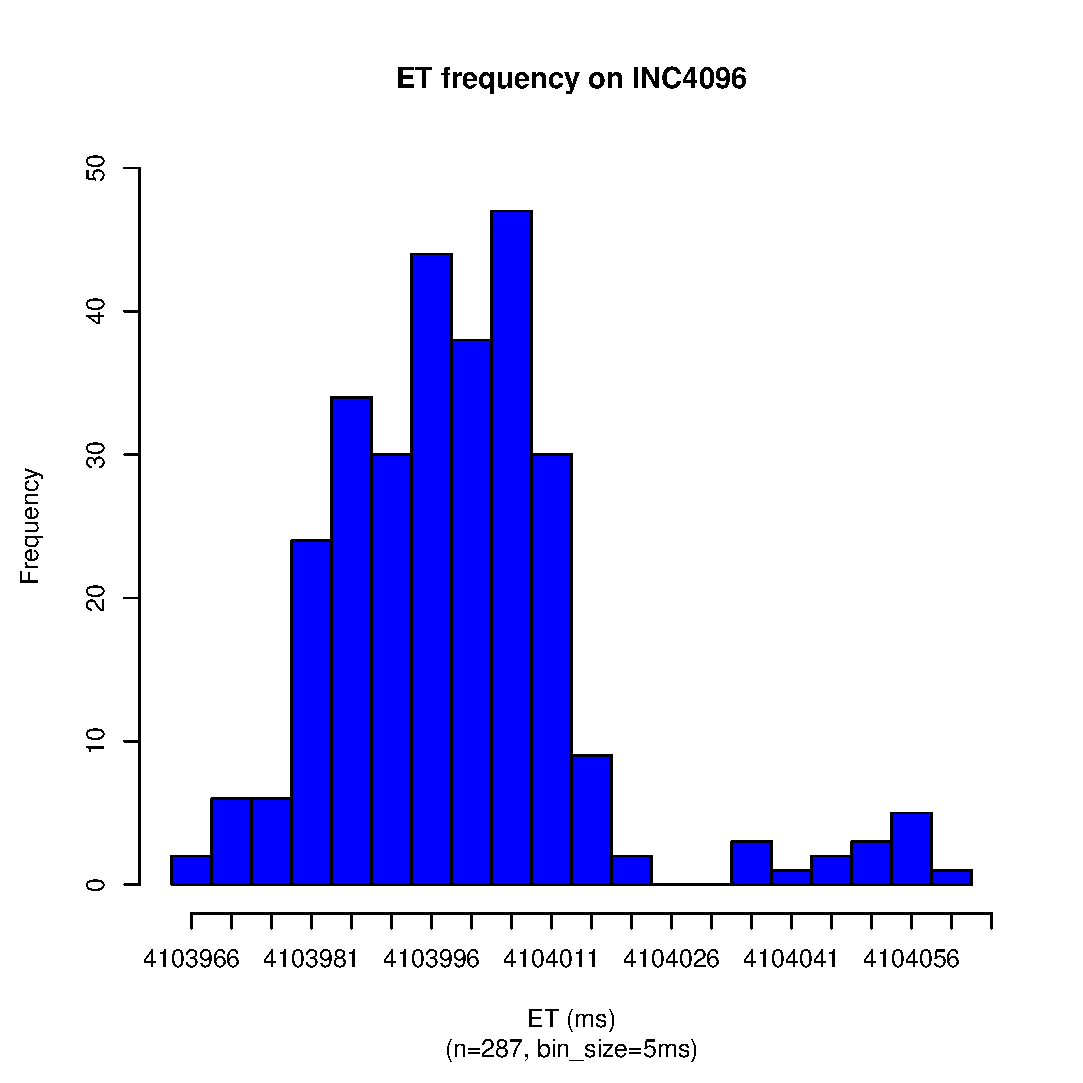
\includegraphics[scale=0.43]{repet_data2/4096_sec_et_hist_v5.eps}
		\label{fig:inc4096_r2_et_hist_v5}
	}
	\caption{ET Histograms of INC2048 and INC4096~\label{fig:s9_r2_et_hist4}}
\end{figure}

\vspace\fill
\clearpage

\subsection{PT}

\begin{figure}[hp!]
	\centering
	\subfigure[PT frequency on INC1]{
		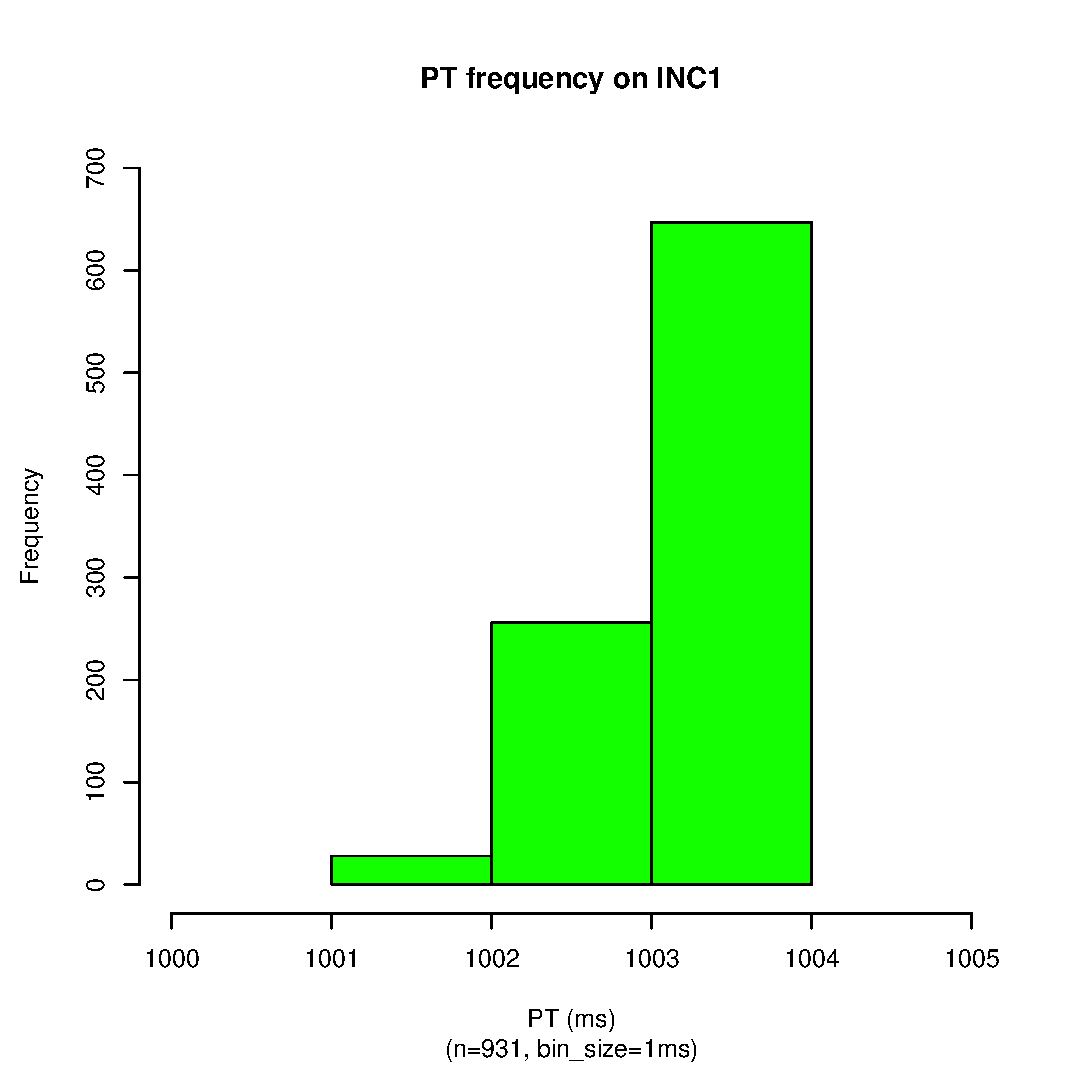
\includegraphics[scale=0.43]{repet_data2/1_sec_pt_hist_v5.eps}
		\label{fig:inc1_r2_hist_v5}
	}
	\subfigure[PT frequency on INC2]{
		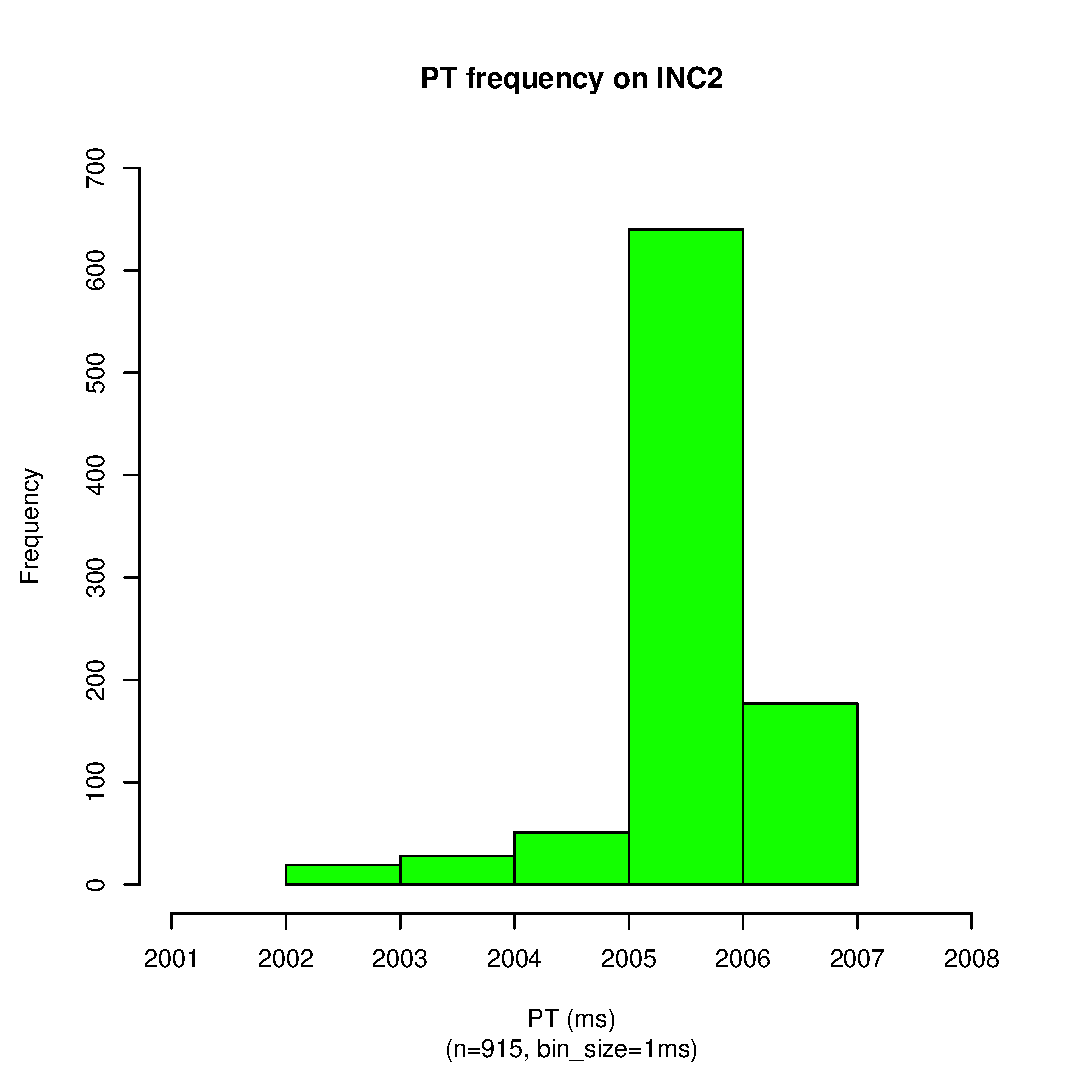
\includegraphics[scale=0.43]{repet_data2/2_sec_pt_hist_v5.eps}
		\label{fig:inc2_r2_hist_v5}
	}
	\subfigure[PT frequency on INC4]{
		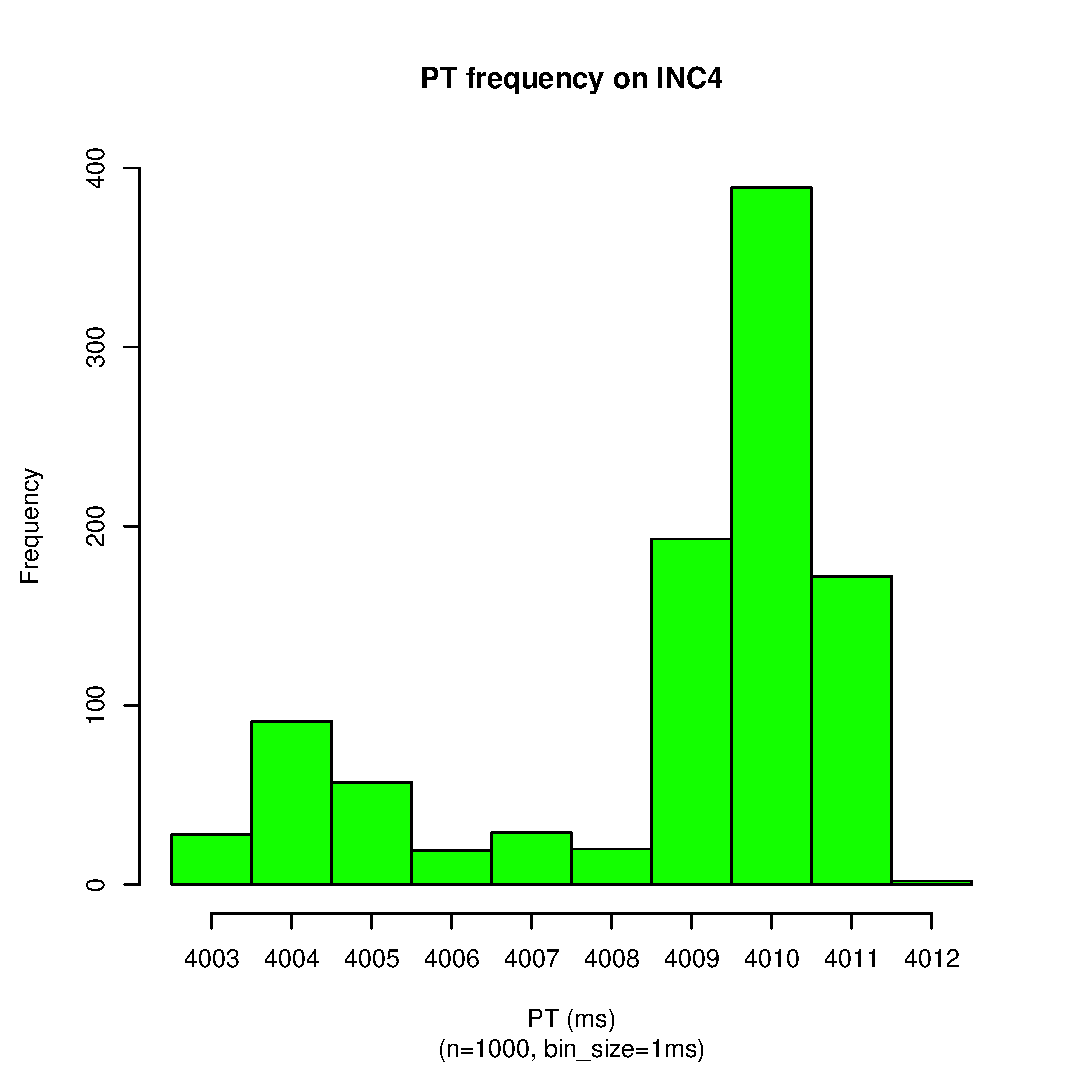
\includegraphics[scale=0.43]{repet_data2/4_sec_pt_hist_v5.eps}
		\label{fig:inc4_r2_hist_v5}
	}
	\subfigure[PT frequency on INC8]{
		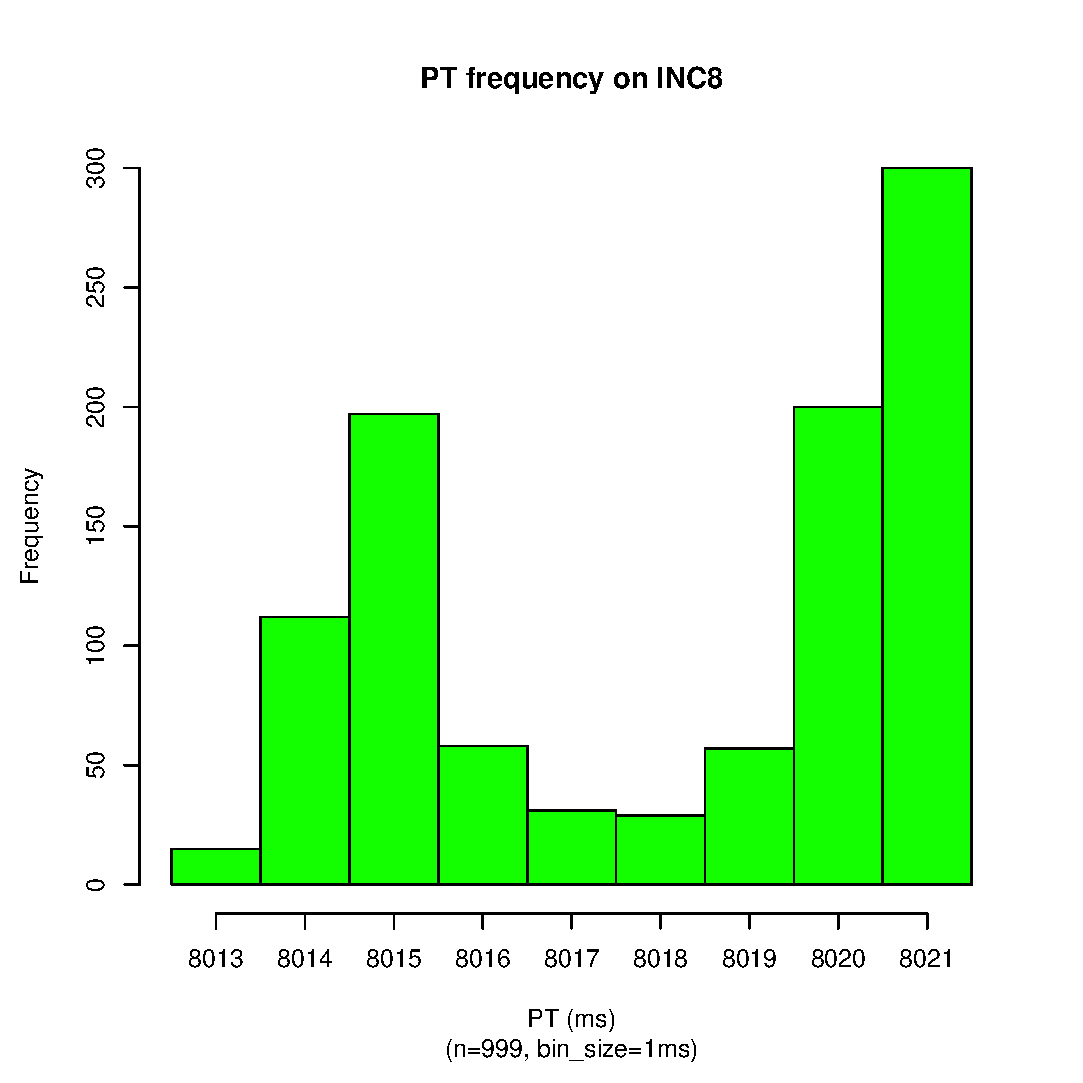
\includegraphics[scale=0.43]{repet_data2/8_sec_pt_hist_v5.eps}
		\label{fig:inc8_r2_hist_v5}
	}
	\caption{PT Histograms of INC1 ... INC8~\label{fig:s9_r2_pt_hist1}}
\end{figure}

\begin{figure}[hp!]
	\centering
	\subfigure[PT frequency on INC16]{
		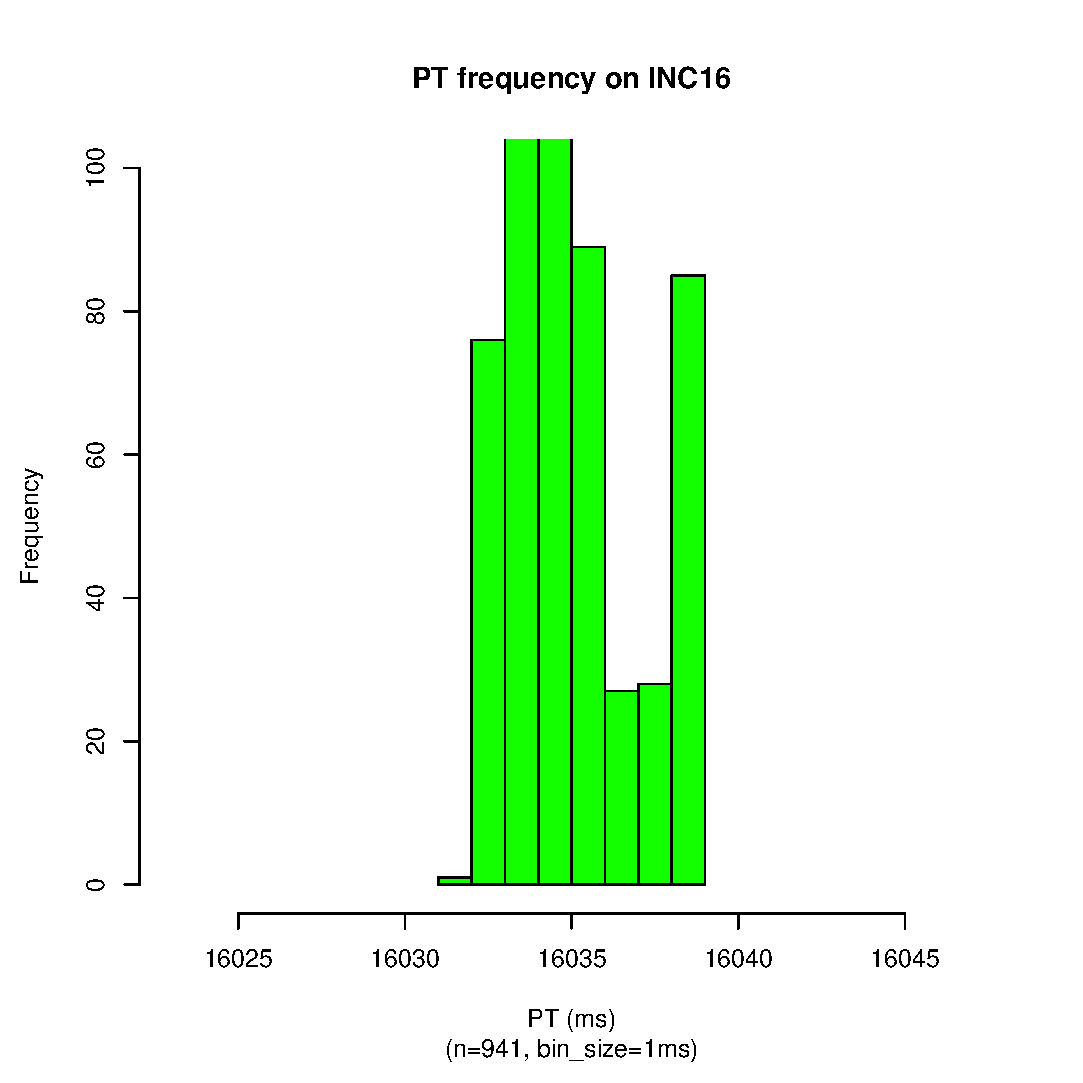
\includegraphics[scale=0.43]{repet_data2/16_sec_pt_hist_v5.eps}
		\label{fig:inc16_r2_hist_v5}
	}
	\subfigure[PT frequency on INC32]{
		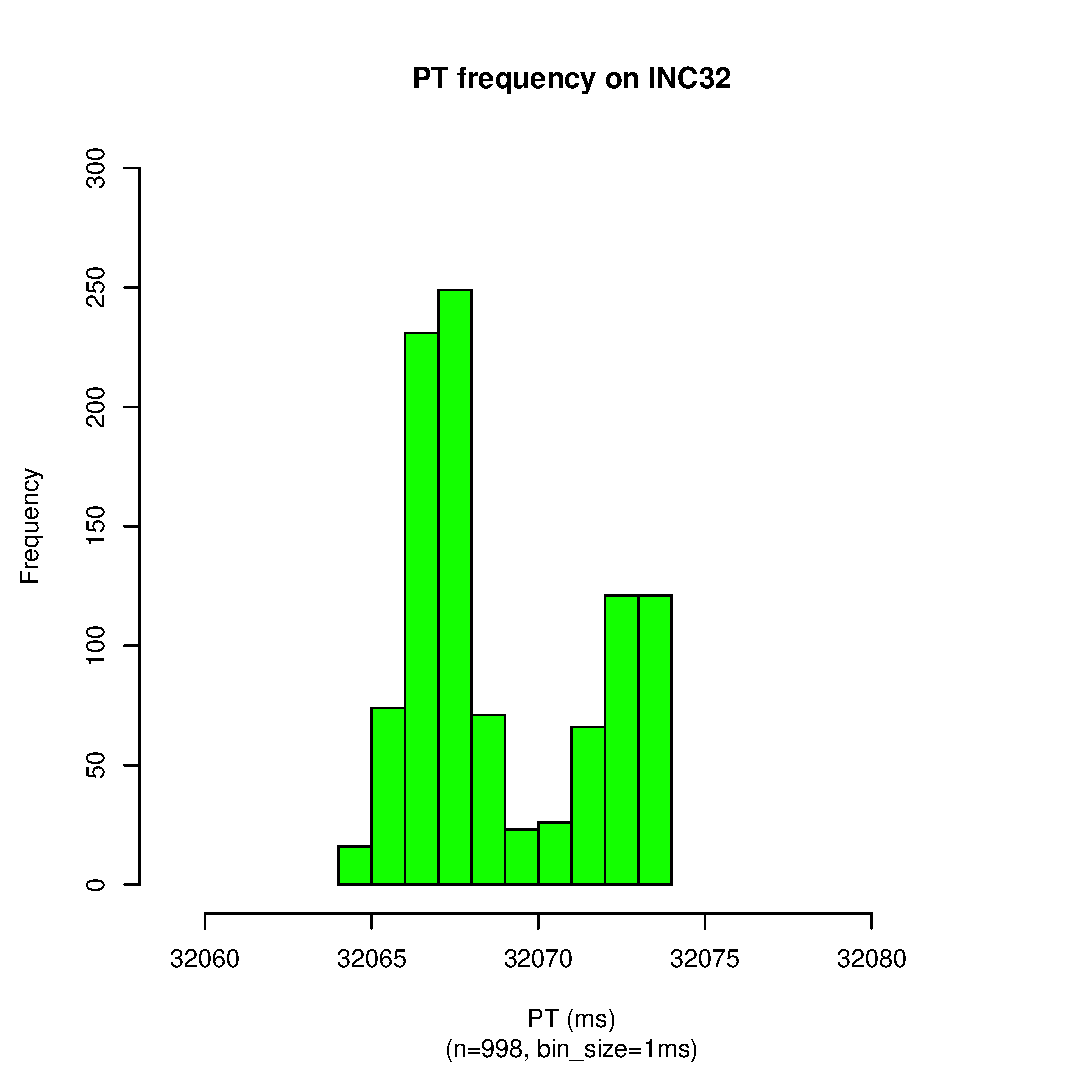
\includegraphics[scale=0.43]{repet_data2/32_sec_pt_hist_v5.eps}
		\label{fig:inc32_r2_hist_v5}
	}
	\subfigure[PT frequency on INC64]{
		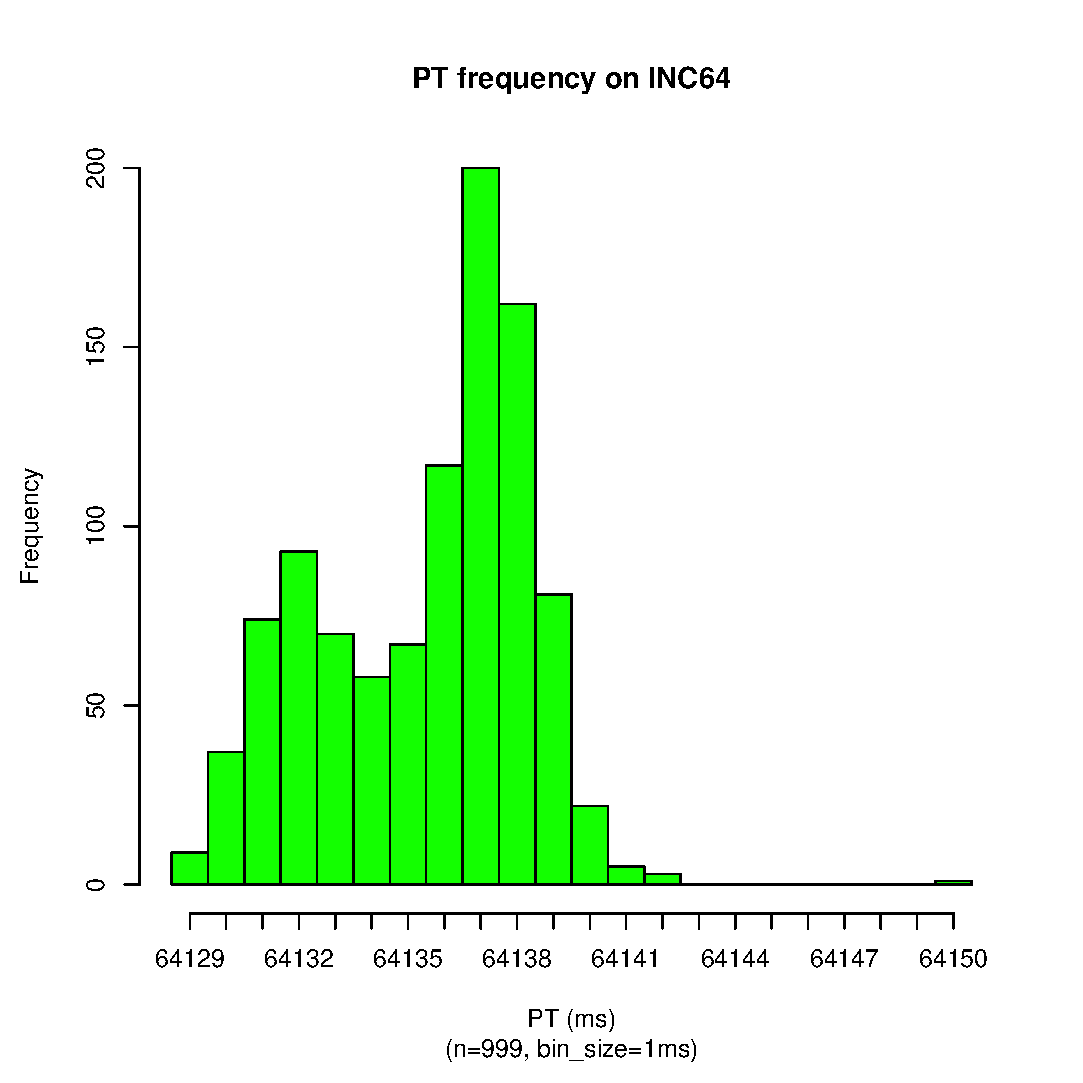
\includegraphics[scale=0.43]{repet_data2/64_sec_pt_hist_v5.eps}
		\label{fig:inc64_r2_hist_v5}
	}
	\caption{PT Histograms of INC16 ... INC64\label{fig:s9_r2_pt_hist2}}
\end{figure}

\begin{figure}[hp!]
	\centering
	\subfigure[PT frequency on INC128]{
		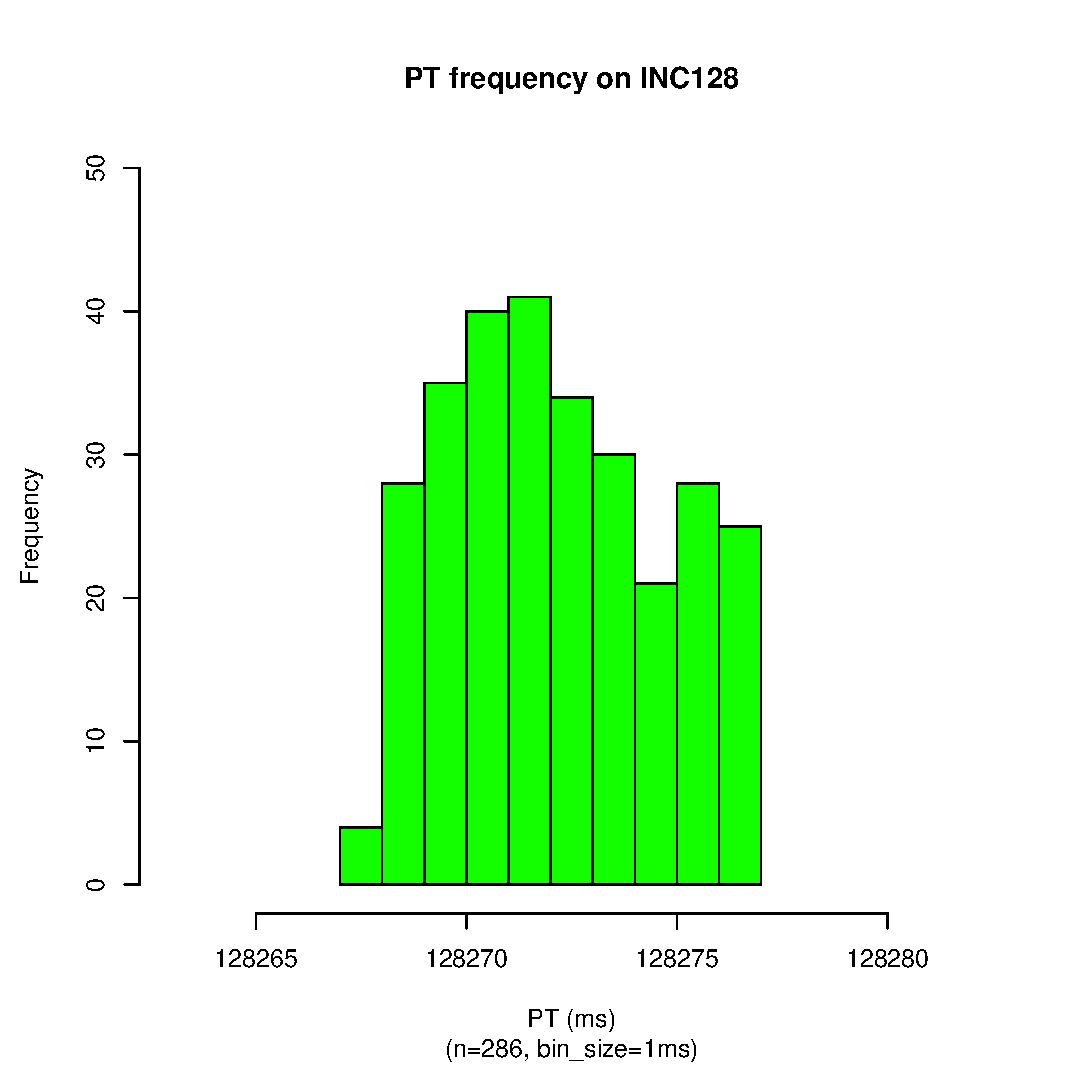
\includegraphics[scale=0.43]{repet_data2/128_sec_pt_hist_v5.eps}
		\label{fig:inc128_r2_hist_v5}
	}
	\subfigure[PT frequency on INC256]{
		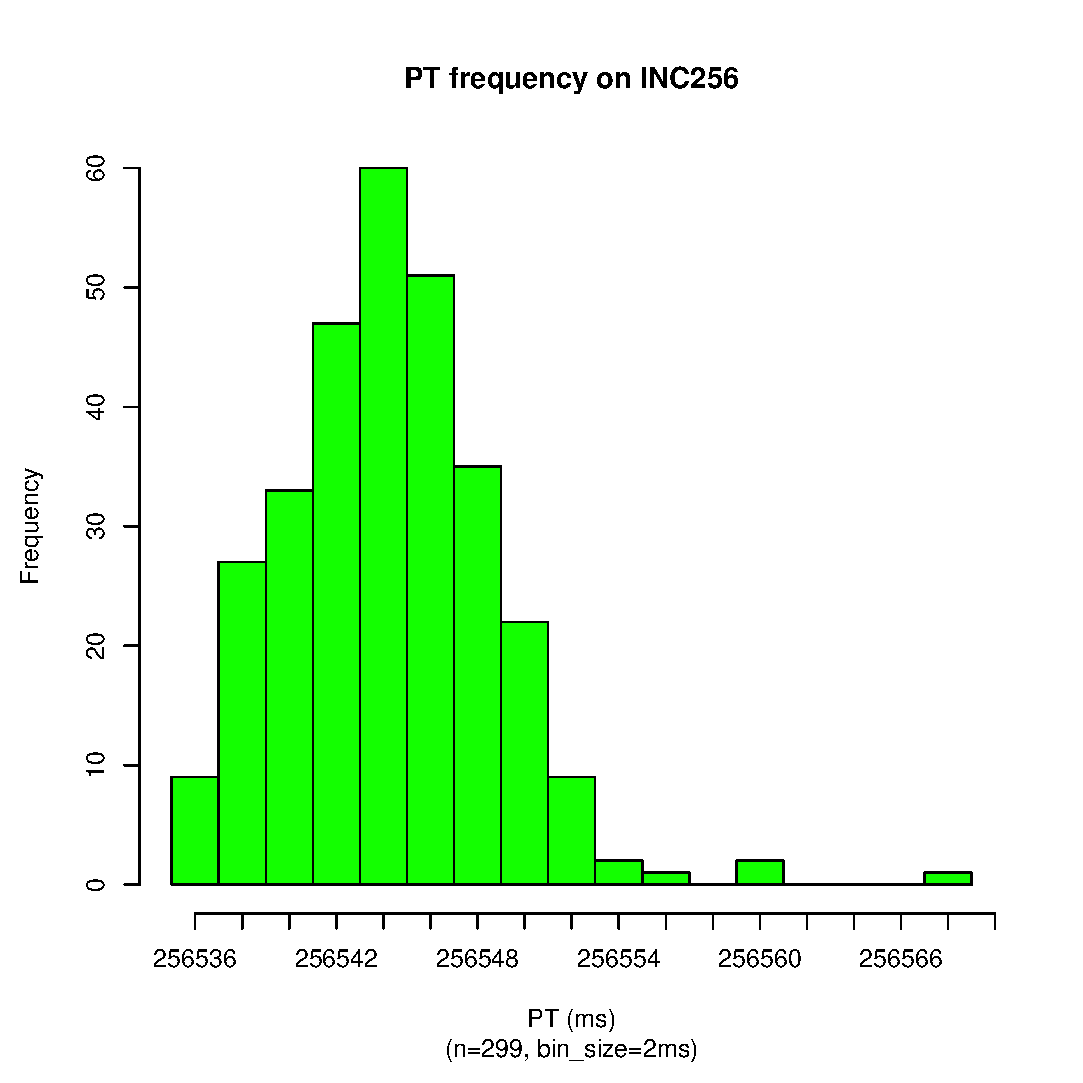
\includegraphics[scale=0.43]{repet_data2/256_sec_pt_hist_v5.eps}
		\label{fig:inc256_r2_hist_v5}
	}
	\subfigure[PT frequency on INC512]{
		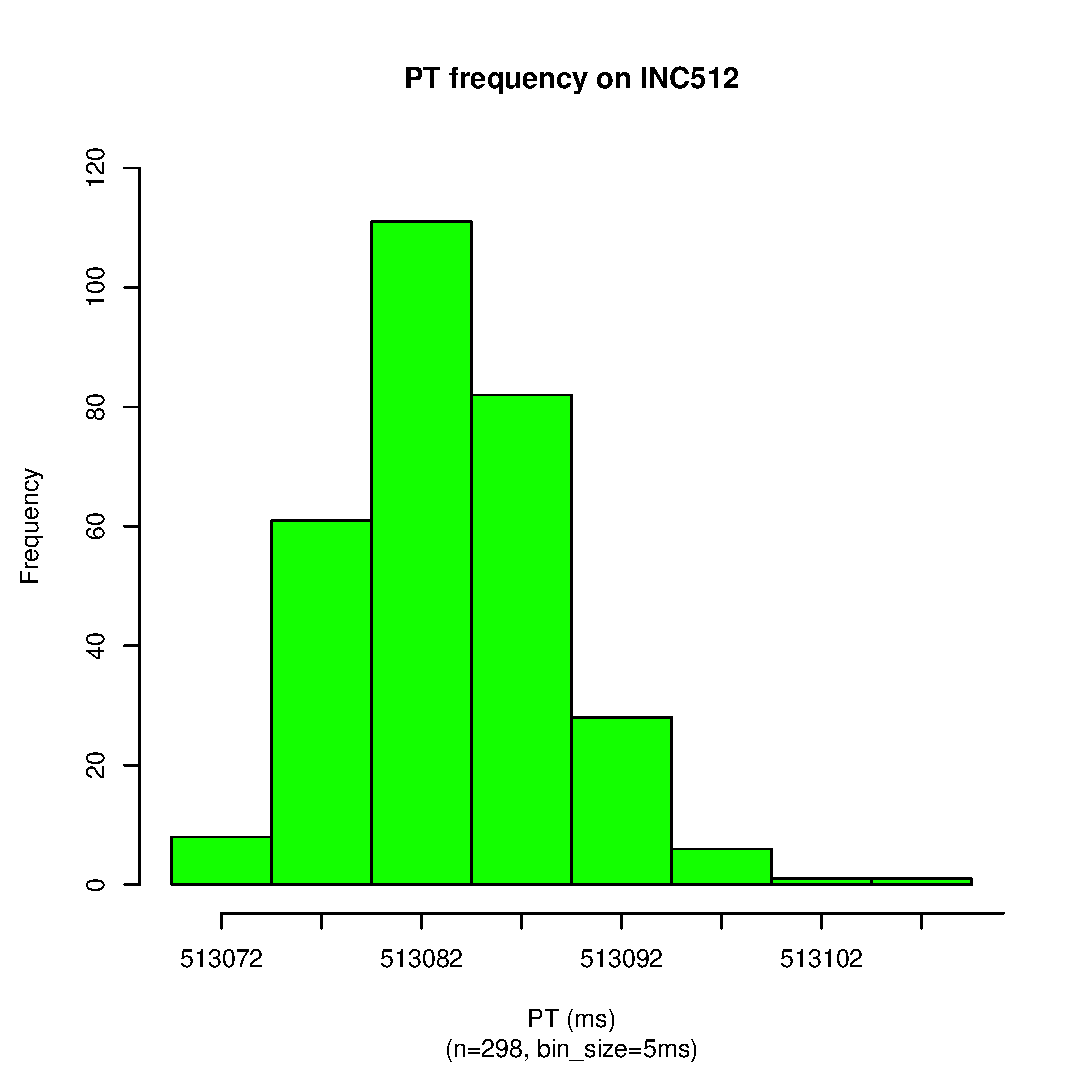
\includegraphics[scale=0.43]{repet_data2/512_sec_pt_hist_v5.eps}
		\label{fig:inc512_r2_hist_v5}
	}
	\subfigure[PT frequency on INC1024]{
		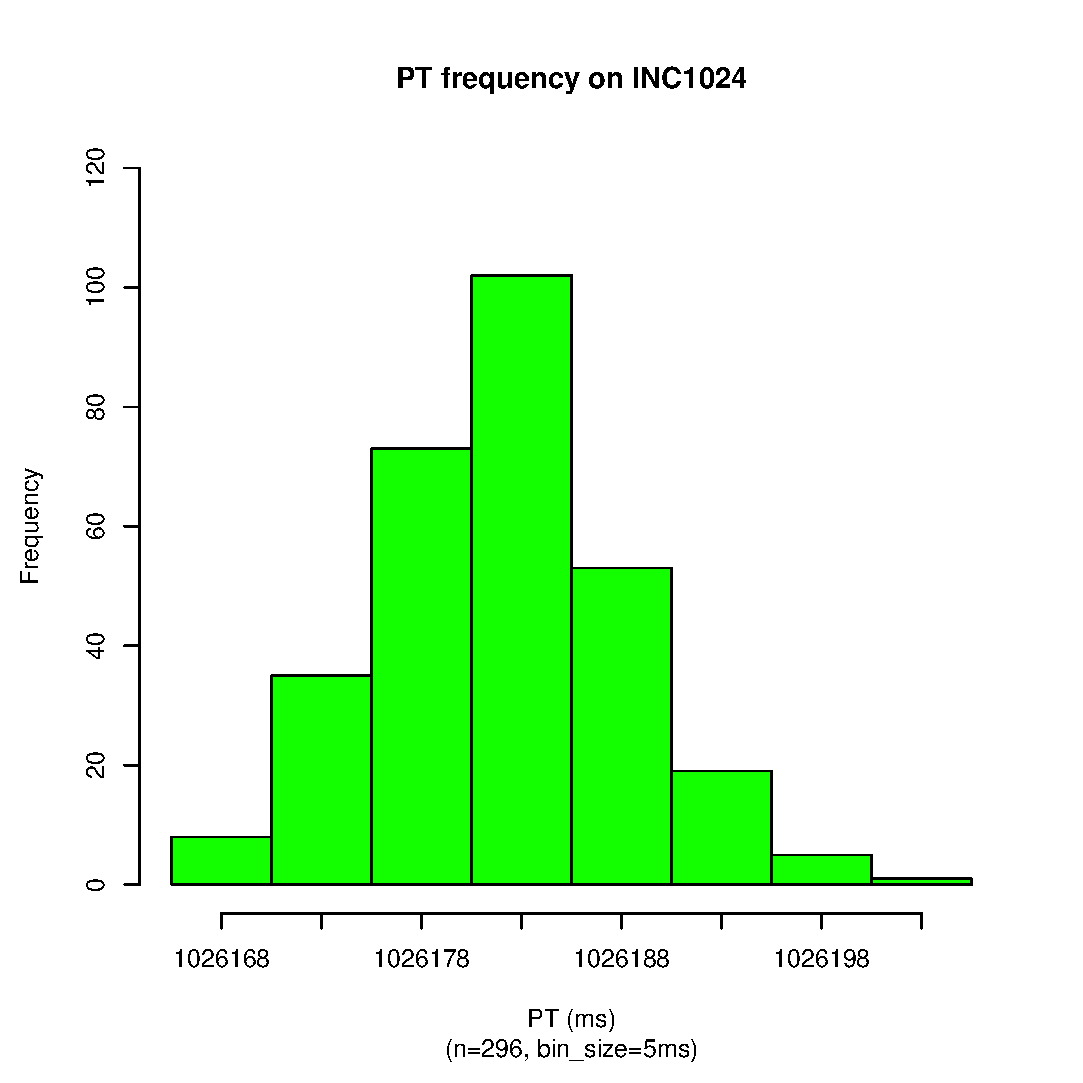
\includegraphics[scale=0.43]{repet_data2/1024_sec_pt_hist_v5.eps}
		\label{fig:inc1024_r2_hist_v5}
	}
	\caption{PT Histograms of INC256 ... INC1024~\label{fig:s9_r2_pt_hist3}}
\end{figure}

\begin{figure}[t]
	\centering
	\subfigure[PT frequency on INC2048]{
		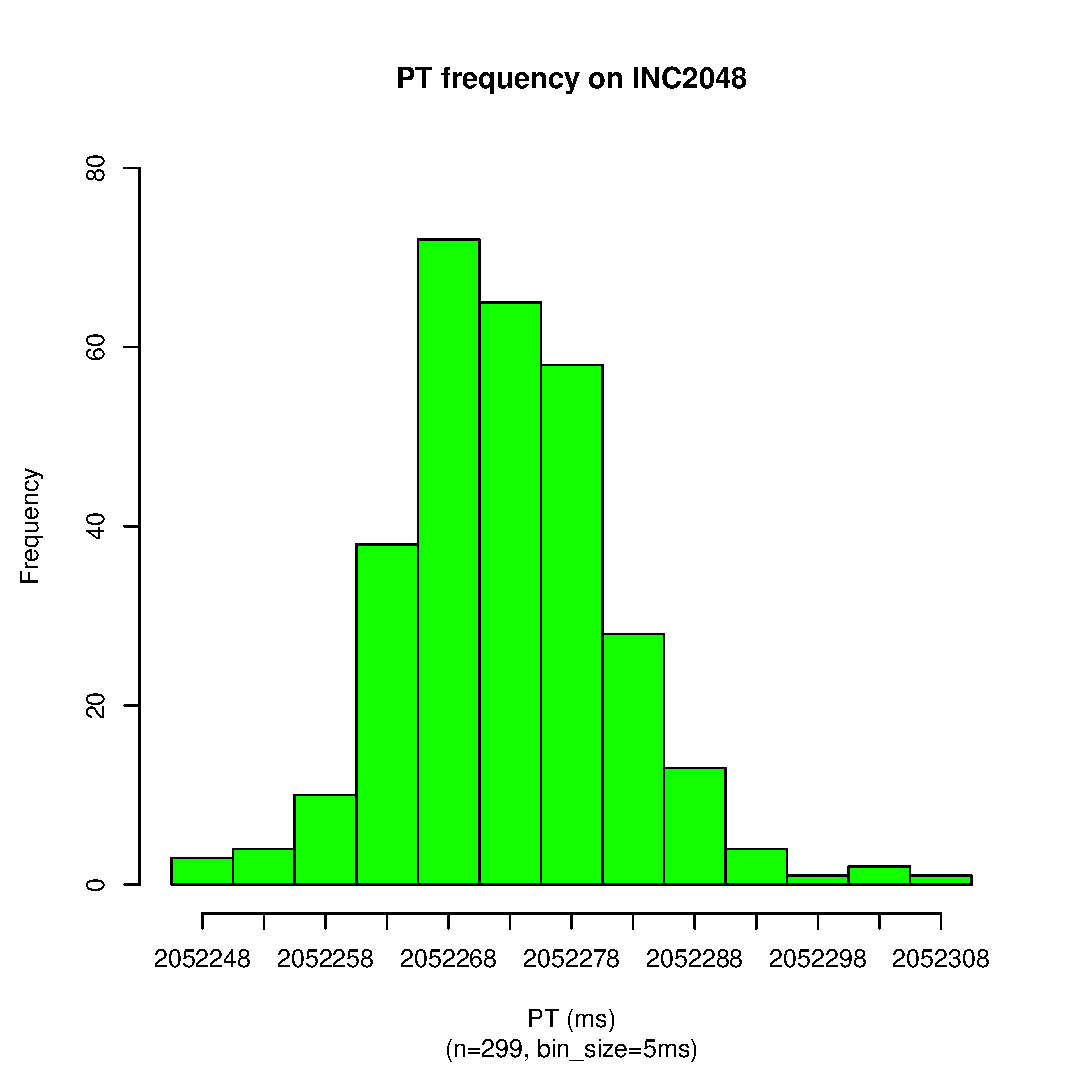
\includegraphics[scale=0.43]{repet_data2/2048_sec_pt_hist_v5.eps}
		\label{fig:inc2048_r2_hist_v5}
	}
	\subfigure[PT frequency on INC4096]{
		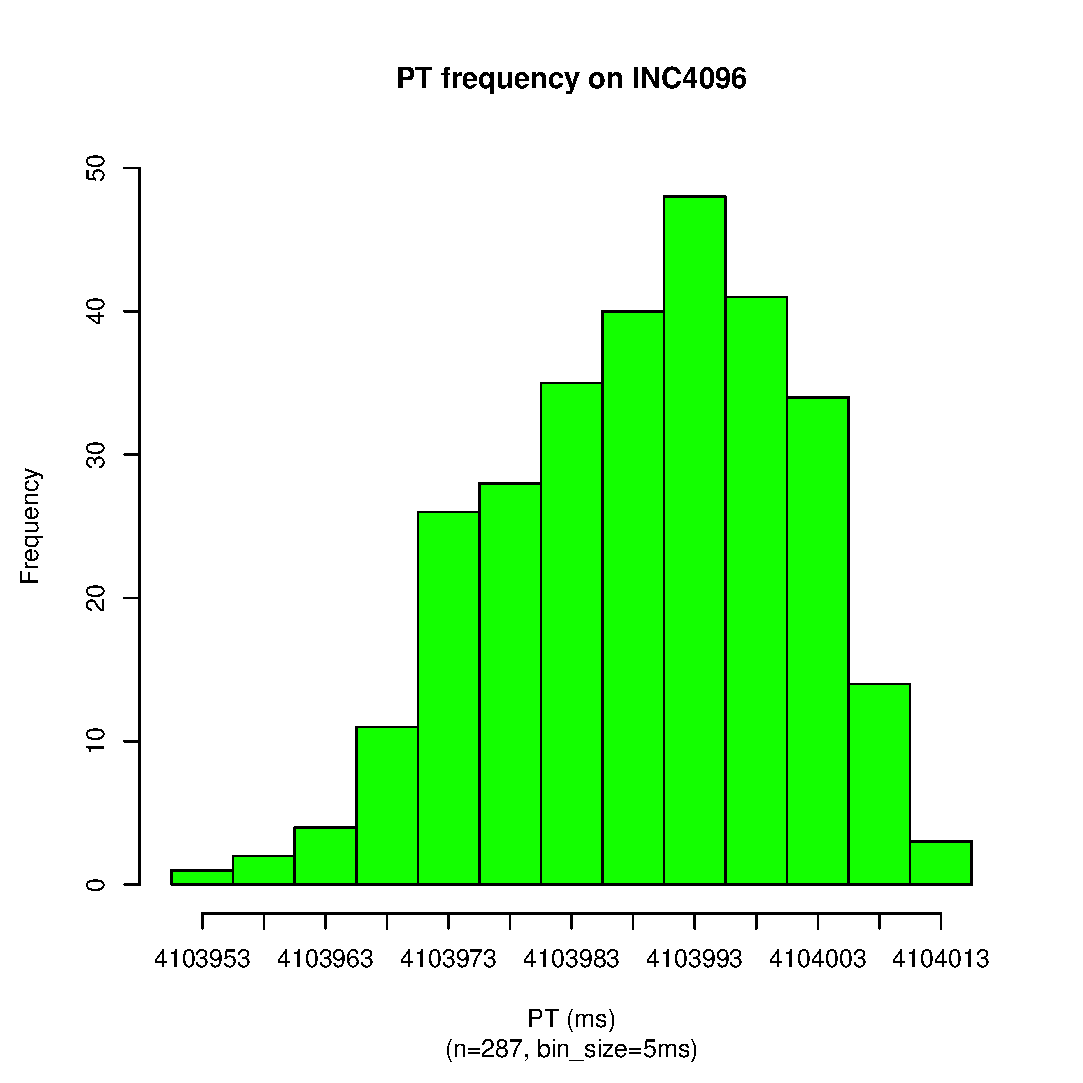
\includegraphics[scale=0.43]{repet_data2/4096_sec_pt_hist_v5.eps}
		\label{fig:inc4096_r2_hist_v5}
	}
	\caption{PT Histograms of INC2048 and INC4096~\label{fig:s9_r2_pt_hist4}}
\end{figure}